 \subsection{Request of selected data of a specific user with subscription, and data visualization}
 
The third part can exploit the Data4Help System, sending a request for the selected data (health data and location) of a specific user, either the last available data, or in subscription mode.  
 In the latter case  it inserts the interval time, i.e. how often wants to receive the updates of these data.
The user can manage his requests, and decide to accept or deny them. If the request is authorized, the third party receives the requested data from the system, according to the chosen modalities.

\begin{table}[H]
	\centering
    
    \begin{tabular}{|p{3.5cm}|p{10.3cm}|}
    
    \hline
    \textbf{\large{Actors}}  			& \tabitem Third part;\tabitem  User  									\\
    				 			
    \hline
    \textbf{\large{Goals}} 				&\ref{goal:user1}; \ref{goal:parties1};\ref{goal:parties2};\ref{goal:parties3}\\
    
    \hline
    \textbf{\large{Enter Condition}} & The third part should be logged in the Data4Help System	\\
    
    \hline
    \textbf{\large{Events Flow}}		& \begin{enumerate}[leftmargin=0.5cm]
                                          	\item The \emph{Third part}  presses the " Request data  from a user" button
                                            \item The \emph{Third part} inserts the specific fiscal code of the target user
                                            \item The \emph{Third part} specifies the parameters that want to receive
                                            
                                            \item The \emph{Third part} can select the subscription mode. If 
                            it is chosen, the third part inserts the interval time. 
                            
                            \item The \emph{System} sends an authorization request to the target user with all the related informations
                                            
                                            \item  The  \emph{user} read the request and accepts it
                                            \item The \emph{System} retrieves the data requested and send them as soon as available to the third part. If the third part has performed a subscription request, it keeps on to send the updated data to the third part how often it has requested.
                                            \item The requested data are shown to the third part
                                
                                          \end{enumerate}
    										\\
    \hline
    \textbf{\large{Exit Condition}} 	& The third part can examine the requested data. \\
    
    \hline
    \textbf{\large{Exception}} 			& -The \emph{target user} denies the request: the negative response is communicated to the third party\newline -The selected fiscal code does not correspond to a registered user:the System asks to insert a validate one.\\
    
    \hline
    
    
    \end{tabular}
	
\end{table}
\begin{figure}[H]
    \centering
    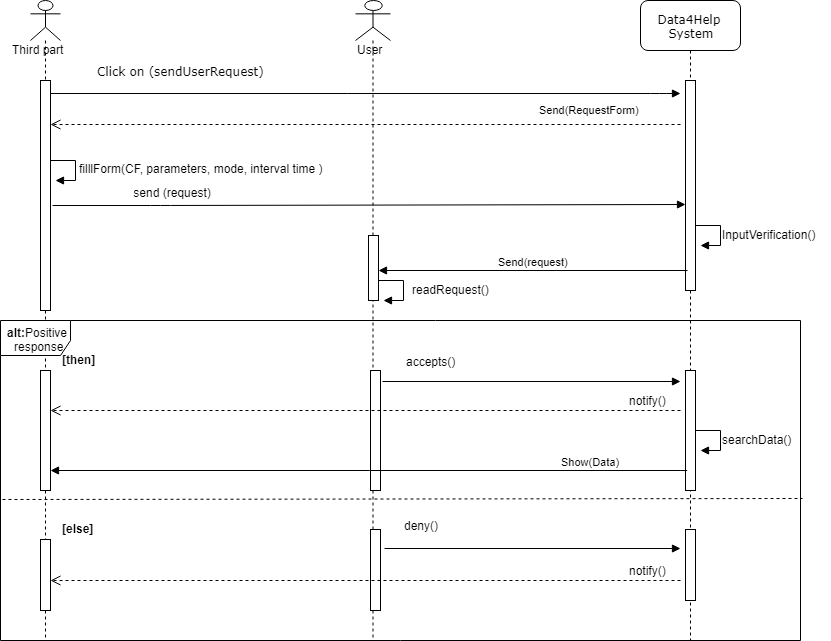
\includegraphics[scale=0.4]{rasdL/Pictures/request1.png}
\end{figure}

